%%% BEGIN CHAPTER 2 MD Simulations and MSM %%%

%% Paper title page %%
\chapter{Molecular dynamics simulations and Markov state modeling of potassium channel monomers}

\section{Introduction}
For oligomeric membrane proteins like potassium channels, the dynamics of monomers are likely to affect the oligomerization process. \textit{In vivo}, the monomers are inserted one at a time from the ribosome-translocon complex, and they must find one another and associate to form native tetramers. Prior to tetramerization, the monomers could be pre-folded in the native-like configuration, or the monomers could exist in a messy heterogeneous ensemble of structure. While the answer to this problem is fundamentally important to addressing the folding of potassium channels, no studies have looked at the dynamics of potassium channel monomers at the atomic-level.

Recently, thiol-labeling experiments demonstrated that the Kv1.3 pore domain monomers immediately begin to form its native-like secondary structures coming out of the ribosome-translocon complex.  \citep{gajewski2011} Through cysteine-scanning experiments, the pore-helix was also shown to maintain its native-like secondary structures. \citep{delaney2014} These studies are the first to show that the pore domain monomers can retain its native-like secondary structures; however, the experiments were not able to resolve what the tertiary structure of the monomer looks like.

In order to address the question of how dynamic is the potassium channel monomer, we use molecular dynamics (MD) simulations and Markov state modeling (MSM) analysis of Kv1.2 and KcsA monomers.

\section{Methods}
\subsection{Preparation of Kv1.2 and KcsA monomer simulations}
For all systems, the initial structures for the monomers were taken from the tetrameric Kv1.2 X-ray crystal structure (PDB ID: 2A79) using only the pore domain of 99 amino acids corresponding to residues 323 –- 421. \cite{long2005} The starting structure for KcsA monomer simulations was taken from the tetrameric KcsA X-ray crystal structure (PDB ID: 1R3J). \cite{zhou2003} All systems were prepared by using CHARMM-GUI’s Membrane Builder module (www.charmm-gui.org). \cite{jo2007, jo2008, jo2009, lee2016, wu2014} For Kv1.2, each system contained 70 palmitoyl-oleoyl-phosphatidylcholine (POPC) molecules per leaflet totaling up to 140 POPC molecules in total, and for KcsA, each system contained 70 1,2-dimyristoyl-sn-glycero-3-phosphatidylcholine (DMPC) molecules per leaflet totaling up to 140 DMPC molecules to match the NMR sample conditions. All systems were hydrated by creating a water box 17.5 \AA \ above and below the protein’s maximum and minimum Z-positions. In addition, all systems were neutralized with 150 mM KCl. Each system comprised a total of approximately 45,000 atoms.

For Kv1.2 simulations, a number of different simulations are aggregated for analysis and they are all summarized in the table below.
\begin{table}[h]
\centering
	\caption{Simulation summary for Kv1.2}
	\begin{tabular}{cccc}
	\hline
    Simulation & Temperature (K) & Number of Trajectories & Trajectory length \\
	\hline                                                                 
	\begin{tabular}[c]{@{}c@{}} Anton\\ simulation \end{tabular} & 353.15  & 1 & 16.2 $\mu$s\\
	GPU & 303.15  & 10 & $\sim$9.7 $\mu$s\\
	\begin{tabular}[c]{@{}c@{}} Adaptive\\ sampling \end{tabular} & 303.15  & 4685 & 0.06$\mu$s\\
	\hline
	\textbf{Total:} & \textbf{N/A} & \textbf{4803} & \textbf{394 $\mu$s}
	\end{tabular}
	\label{table:ch2_t1}
	\end{table}
	
For KcsA simulations, 5 independent simulations of KcsA WT monomer were carried out at T = 353 K to enhance sampling. All simulations were run with the parameters described in \textit{Amber16 simulations} section below, and each simulation was run up to 6 $\mu$s. In total 30 $\mu$s of KcsA WT simulations were accumulated.

\subsection{Anton simulations}
A long-time simulation run on Anton \cite{shaw2009} was prepared through energy minimization and equilibrating the initial simulation system using CHARMM36 force field with NAMD. \cite{phillips2005} Each system was energy minimized for 1,000 steps and was slowly equilibrated by reducing restraints on protein backbone, sidechain, and lipids gradually over 5 ns as recommended by CHARMM-GUI. After initial equilibrations with the restraints, the system was freed from all restraints and run for 100 ns before preparing the system for running simulations on Anton. The temperature was set to 353 K to increase sampling, which has been shown to capture thermodynamics more computationally efficiently. \cite{ulmschneider2014} All bonds involving hydrogen atoms were constrained by M-SHAKE. Cut-off values for van der Waals and short-range electrostatic interactions were optimized by Anton guesser script. For long-range electrostatic interaction calculations, k-space Gaussian split Ewald method with a 64 x 64 x 64 mesh was used, and the long-range electrostatics were calculated every 6 fs. The integration time step was 2 fs for all simulations, and the r-RESPA integration method was employed. \cite{tuckerman1992}

\subsection{Amber16 simulations}
For all systems that were simulated with Amber16 GPU, hydrogen mass repartitioning (HMR) scheme was applied, where all hydrogen masses were increased to 3, allowing simulation timestep to increase from 2 to 4 fs. The systems were prepared as described in System Preparation section using CHARMM-GUI, and \textit{parmed.py} program was used to modify the system to accommodate the HMR scheme. For temperature control, Langevin thermostat was used with friction coefficient of 0.3 and T=303 K, and coordinates were printed out every 50 ps. van der Waals force switching function was used with switch on at 10 Å and cutoff at 12 Å. Berensden barostat is used with semi-isotropic at pressure 1 atm. The Berensden coupling constant is set to 0.5 ps.

\subsection{Markov state model (MSM) analysis}
For all molecular dynamics (MD) simulation analysis, MDTraj 1.9.0 and MSMbuilder 3.8.0 were used. \citep{harrigan2017, mcgibbon2015} In the first steps of constructing a Markov State Model (MSM), proper set of reaction coordinates, and discretized states within the chosen reaction coordinates are needed. For these purposes, time-lagged independent component analysis (TICA) and K-Center clustering algorithm were used.

\subsubsection{Time-lagged Independent Component Analysis (TICA)}
TICA is a method that was first used in the signal processing community \citep{molgedey1994} and was later introduced to the molecular dynamics community by two independent research groups. \citep{perezHernandez2013, schwantes2013} TICA was introduced as a method to extract slow order parameters, and because most interesting protein motions are thought to be the slowest in timescaale, TICA is excellent for discovering important reaction coordinates.

TICA shares a lot of similarity to principal component analysis (PCA). In PCA, the projection vectors that maximize the explained variance is found by solving the generalized eigenproblem of the covariance matrix. 

\begin{equation}
\Sigma \nu = \lambda \nu
\end{equation}

where the covariance matrix is given by:

\begin{equation}
\Sigma_{ij} = \mathbb{E} \Big[X_{i}(t)X_{j}(t)\Big]
\end{equation}

In biomolecular simulations, PCA can be useful when the system of interest needs a reaction coordinate that corresponds to the largest motions in the simulations. However, often times, the largest motions in the biomolecular simulations do not necessarily correspond to the most interesting protein motions. TICA complements this problem by solving the generalized eigenproblem of the auto-correlation matrix of the dynamic system. For TICA, we solve the generalized eigenproblem defined as:

\begin{equation}
C^{(\Delta t)} \nu = \lambda \Sigma \nu
\end{equation}

where

\begin{equation}
C_{ij}^{(\Delta t)} = \mathbb{E} \Big[ X_{i}(t)X_{j}(t+\Delta t)\Big]
\end{equation}

In practice, for TICA, a set of relevant features must be inputted to generate a set of low-dimensional linear combination of the input features. Common input features include pair-wise C-$\alpha$ distances, inverse distances, and dihedral angles. For our system, pairwise distances of all C-$\alpha$ atoms of all residues were used, which resulted in 4,831 total features. Then through TICA, dimensionality reduction was performed. Based on implied timescale analysis, 3 TICs with the slowest relaxation timescale was found to adequately describe our system (\textbf{Fig. \ref{fig:ch2_f1}}). Then, all simulations were transformed and projected onto the 3 TICs found.

\begin{figure}[!ht]
\begin{center}
	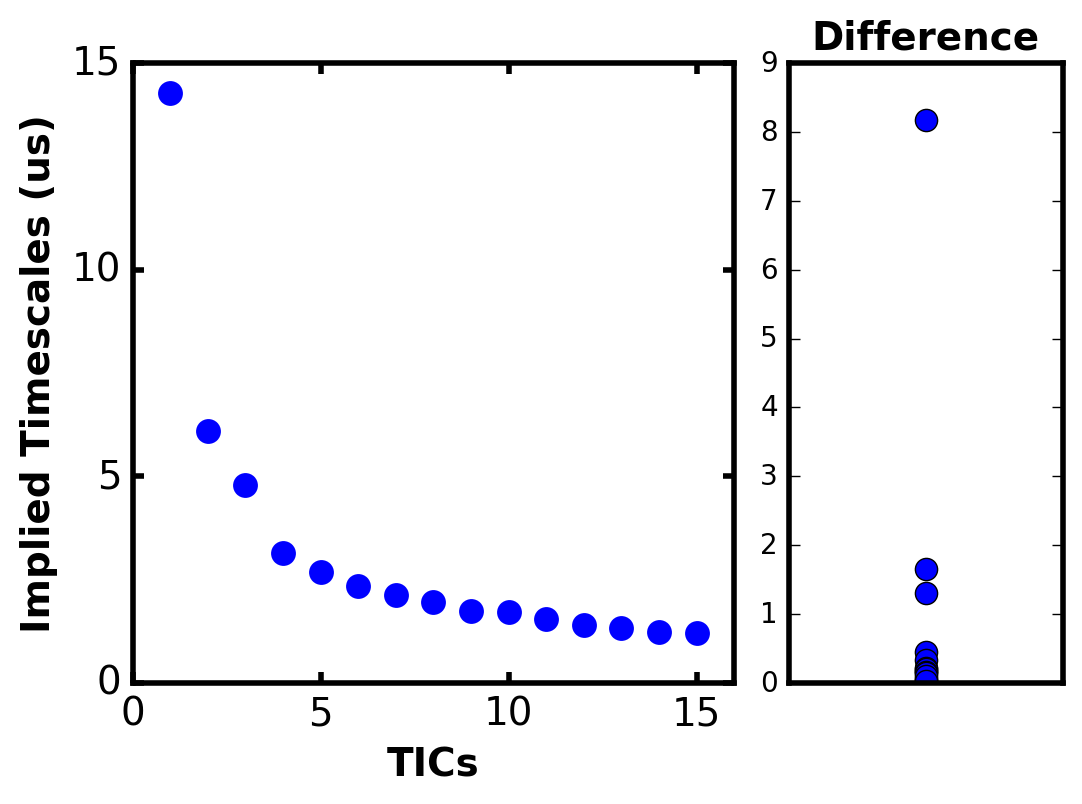
\includegraphics[width=13cm]{figures/chapter2/Fig2-1_implied_timescale.png}
\end{center}
	\caption{\textbf{TICA analysis of Kv1.2 simulations.} The implied relaxation timescale of each TIC is plotted versus the number of TICs. The first 3 TICs are chosen as reaction coordinates to represent the folding coordinates of the simulations.}
	\label{fig:ch2_f1}
\end{figure}

\subsubsection{K-Center clustering}
To discretize a set of relevant conformations within the TIC space, K-Center clustering algorithm was used. K-Center clustering algorithm is an unsupervised machine learning method, where given k number of states, the algorithm learns to find k cluster centers that minimize the distances between the data point and its corresponding cluster center. Initially, the cluster centers are randomly chosen, and each data point is assigned to its closest cluster center based on distance. Then, new cluster centers are updated by finding data point closest to the average of each cluster. The process of assigning data to clusters and updating cluster centers are repeated until convergence.

\begin{figure}[!ht]
\begin{center}
	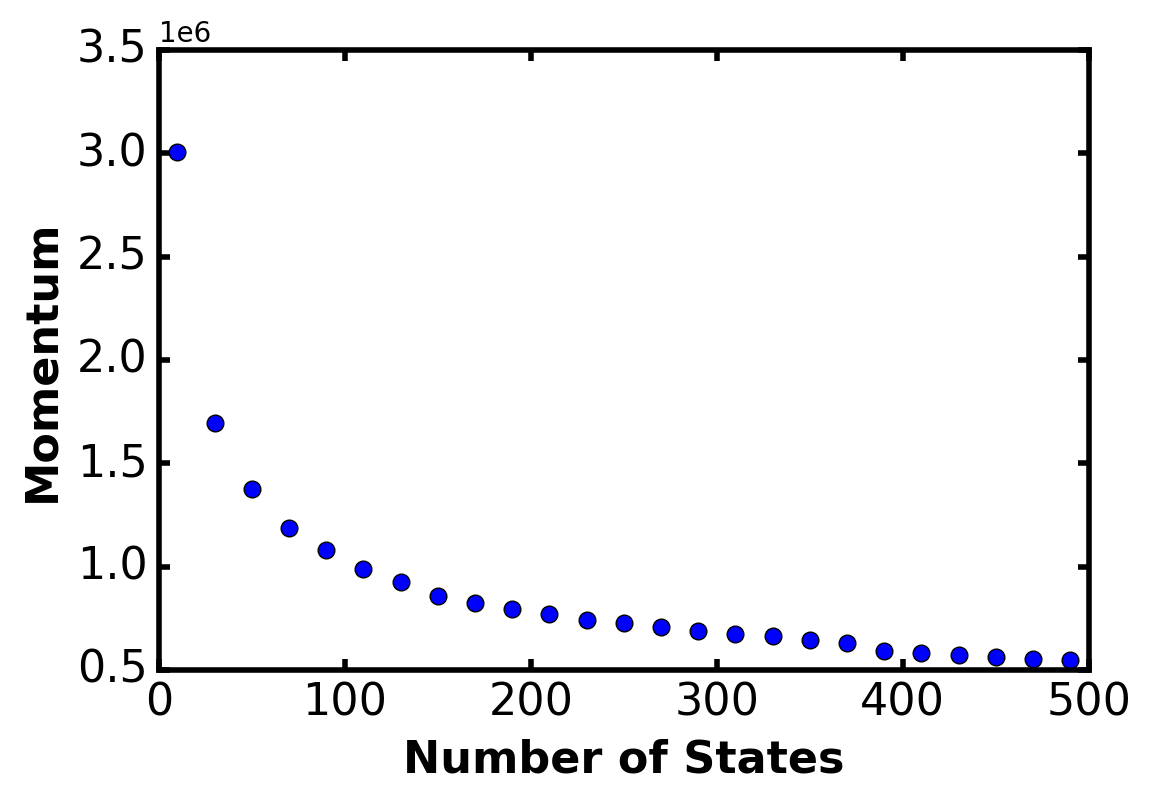
\includegraphics[width=13cm]{figures/chapter2/Fig2-2_momentum.png}
\end{center}
	\caption{\textbf{Change in momentum over number of states.} Momentum is calculated as the sum of distances between each data point and its nearest centroid. To determine the optimal number of states for K-Center clustering method, the number of states where the momentum value begins to plateau is chosen. For our studies, k=150 states deemed to be optimal.}
	\label{fig:ch2_f2}
\end{figure}

In practice, finding the optimal number of states for K-Center clustering is empirically determined. The number of states is determined using the elbow method, where the momentum (sum of squared distances of samples to their closest centers) is plotted against the number of states. The number of states where the decrease in inertia became marginally less than a certain threshold is found. For Kv1.2, k=150 states was found to be appropriate for clustering (\textbf{Fig. \ref{fig:ch2_f2}}).

\subsubsection{Markov State Model (MSM) analysis}
Markov state models (MSMs) are a class of discrete, kinetic model that is largely based on Markov chains. MSMs assume that the system is memoryless and jump from one state to another purely based on its transition probabilities. In order to create a robust MSM, one must find a set of discrete conformational states and estimate the transition probabilities between each state. Previously through TICA and K-Center clustering algorithm, a set of microstates were found. Next, the transition matrix must be estimated through the count matrix and maximum likelihood algorithm.

For the count matrix \textbf{C}, C$_{ij}$ is calculated by counting the number of times a transition is made between states i and j given time $\Delta$t


\subsection{Adaptive sampling scheme}
For adaptive sampling, initial MSM was constructed using only the Anton trajectory. Adaptive sampling scheme described previously by Bowman et. al was used. \citep{bowman2010} In each round of simulations, 50 states with the lowest MSM populations are chosen and those chosen centroid conformations are used as seeds for additional 60 ns of AMBER16 simulations using the CHARMM36 force field with Hydrogen Mass Repartitioning (HMR) scheme. After each round of simulations, new sets of TICs are calculated and a new MSM is constructed. This method allows better sampling of states with low transition probabilities and help refine the total free energy landscape. In total, we accumulated 394 $\mu$s of simulations which are then used to create the final MSM for WT Kv1.2 monomer. 

\section{Results and Discussion}
\subsection{Potassium channel monomers are dynamical}
In a previous 650 ns MD simulation, the wild-type (WT) Kv1.2 pore domain monomer in POPC lipid bilayer was stable in a native-like state with a C$\alpha$-RMSD below 3 \AA. \cite{gajewski2011} However, this simulation is relatively short compared with the micro- to the millisecond timescale of membrane protein dynamics. \citep{booth1995} To further explore the monomer’s conformational flexibility, we carried out 16.2 $\mu$s of simulations at T=353 K using the specialized Anton computer designed for simulations.\citep{shaw2009} The relatively high temperature was chosen to accelerate sampling while still reproducing the thermodynamics of membrane protein folding.

\begin{figure}[!ht]
\begin{center}
	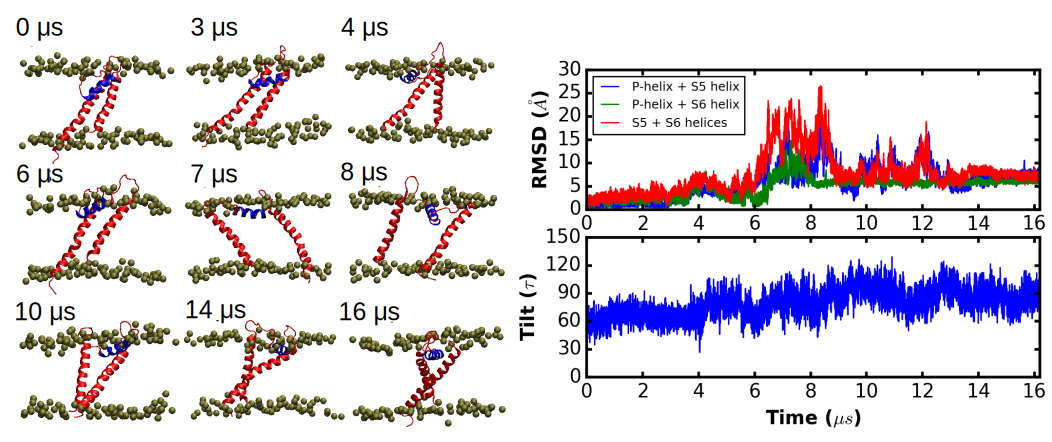
\includegraphics[width=\textwidth]{figures/chapter2/Fig2-3_anton.pdf}
\end{center}
	\caption{\textbf{Molecular dynamics simulation of Kv1.2 pore domain monomer in POPC lipid bilayer ran for 16.2 $\mu$s on Anton.} \textbf{Left}: Selected snapshots. \textbf{Right}: Pair-wise C$\alpha$-RMSD values for pairs of helices and the tilting angle of the pore helix.}
	\label{fig:ch2_f3}
\end{figure}

During the first 3 $\mu$s of the simulation, the structure was stable with a C$\alpha$-RMSD to the initial (native-like) state below 4 \AA \ (\textbf{Fig. \ref{fig:ch2_f3}}). Nevertheless, the p-helix became more parallel to the membrane during the first microsecond with the tilt angle increasing from 47$^{\circ}$ to 80$^{\circ}$ relative to the surface normal (\textbf{Fig. \ref{fig:ch2_f3}}). The average tilt angle over the entire 16.2 $\mu$s was 80$^{\circ}$ $\pm$ 10$^{\circ}$. At 4 $\mu$s, the 2 TM helices started to separate laterally with slightly different tilt angles due to their different lengths, leading to overall C$\alpha$-RMSD values greater than 4 \AA. 

Between 6 and 8 $\mu$s, all three helices separated (Fig. S1), but the p-helix remained helical and stayed nearly parallel to the membrane surface. This orientation allowed the polar and charged residues in the pore loop region to become more solvent exposed, while segregating the nonpolar residues. This result is qualitatively consistent with the previous thiol-labeling results, which indicated that the p-helix remains helical and resides at the water-lipid interface. \citep{delaney2014} Based on short simulations (650 ns) and thiol-labeling experimental data, the Kv1.3 monomer was inferred to retain native-like tertiary contacts. \citep{gajewski2011} In the long Anton simulation, however, the monomer is stable up to 3 $\mu$s with RMSD less than 4 \AA  \ but also explores many other non-native states.

\begin{figure}[!ht]
\begin{center}
	\includegraphics[width=\textwidth]{figures/chapter2/Fig2-4_saltbridge.pdf}
\end{center}
	\caption{\textbf{Intra-monomer salt-bridge mimics a native inter-monomer salt-bridge.} \textbf{Top}: Snapshots from the simulation are shown from the side and from the top with D363 highlighted in red and K388 highlighted in blue. \textbf{Bottom}: left cartoon shows the rearrangement of the inter-monomer salt-bridge to an intra-monomer salt-bridge. Right figure shows the native inter-monomer salt-bridge interaction.}
	\label{fig:ch2_f4}
\end{figure}

After 8 $\mu$s of simulations, residue D381 formed a salt bridge with a K398 that resides on top of the carboxy-terminal S6 helix (\textbf{Fig. \ref{fig:ch2_f4}}). This salt bridge persisted for the last 8 $\mu$s and stabilized the interactions between the S6 and the p-helix. The amino terminal S5 helix eventually drifted towards the complex formed by the S6 with the p-helix, to produce an alternate structure. Interestingly, the salt bridge formed between the p-helix and S6 mimics a salt-bridge that is formed between p-helix of one monomer with the S6 helix of an adjacent monomer in the native tetramer (which does exist in the simulations). Salt bridges are known to be overly stabilized in simulations \citep{ahmed2018} so the longevity of the D381-K398 bridge may be unrealistic. Nevertheless, the monomer spent a majority of time with the three helices in a non-native arrangement.

\subsection{Markov state modeling of Kv1.2 and KcsA monomer simulations}
To obtain a better estimate of the conformation ensemble of Kv1.2 monomers, an analysis based on Markov state models (MSM) was performed using 3 sets of simulations (\textbf{Table. \ref{table:ch2_t1}}): (1) 16.2 $\mu$s Anton simulation at T=353 K; (2) 10 independent 9 $\mu$s long simulations starting from the native state at T=303 K; (3) 100 rounds of adaptive sampling simulations (SI Methods) at T=303 K. A total of 394 $\mu$s of simulations was accumulated and used for time-structure Independent Component Analysis (TICA) and MSM analysis. \citep{molgedey1994, noe2015, noe2016, perezHernandez2013, schwantes2013}

\begin{figure}[!ht]
\begin{center}
	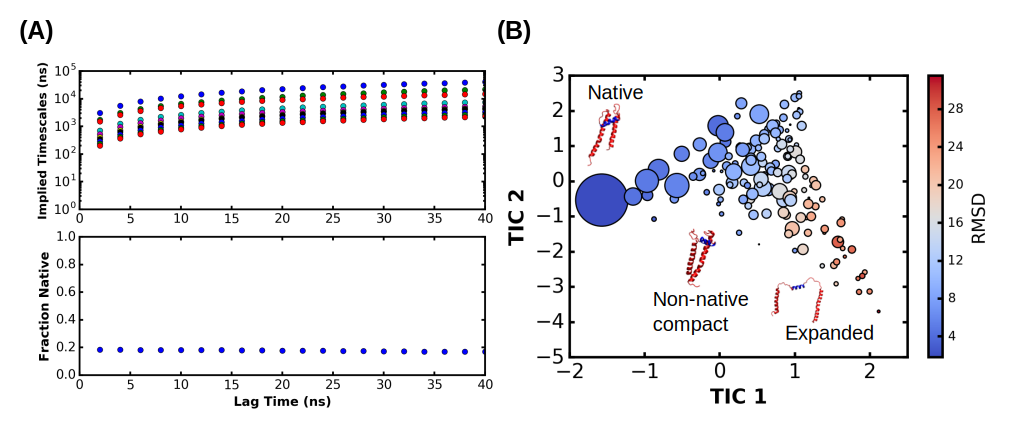
\includegraphics[width=\textwidth]{figures/chapter2/Fig2-5_msm.pdf}
\end{center}
	\caption{\textbf{MSM built on 394 $\mu$s of total simulation time at 303 K.} \textbf{(A) Top}: Implied timescale analysis of Markov State Model. \textbf{Bottom}: Lag-time analysis of fraction native indicates that 18\% of the population remains native-like. \textbf{(B)} Markov state model built with lag time of 20 ns is projected onto TIC1 and TIC2. The size of the circle is proportional to the population of each microstate and the color of the circle represents the RMSD of each microstate to the native structure (in the tetramer).}
	\label{fig:ch2_f5}
\end{figure}

Based on the MSM analysis, the population of native-like structures (C$\alpha$-RMSD < 4 Å) converged at 18\% (\textbf{Fig. \ref{fig:ch2_f5}A Bottom}). This result further supports the finding that the native-like monomer conformation is present but is not predominant in lipid bilayer. While the two TM helices and the p-helix retained their helicity in all structures, the monomer prefers to be partially disordered. The p-helix remained parallel to the water-lipid interface, which is consistent with the thiol-labeling results. \citep{gajewski2011} Overall, the monomer existed as a heterogeneous ensemble of contacting and non-contacting helices.

\subsection{Kv1.2 and KcsA monomers show similar behavior}

\begin{figure}[!ht]
\begin{center}
	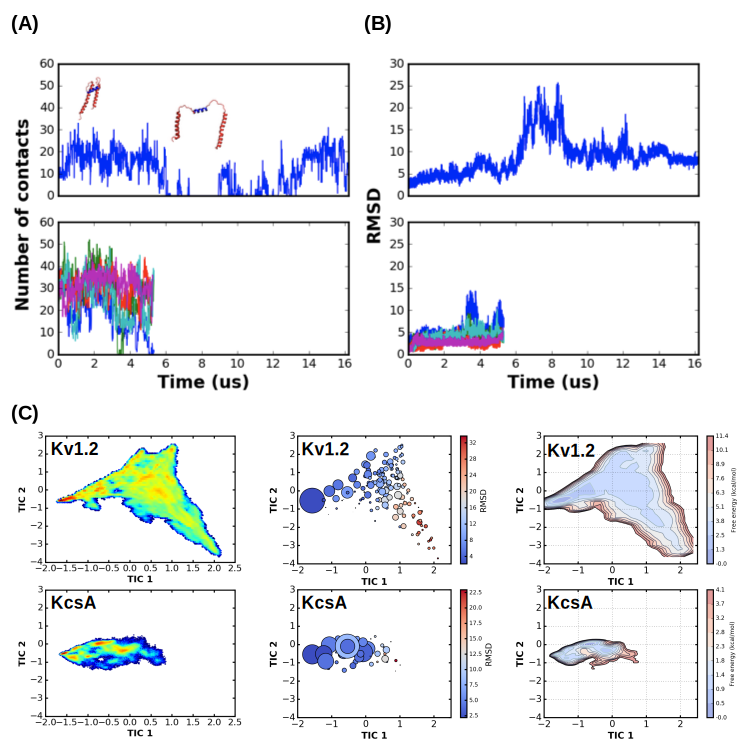
\includegraphics[width=\textwidth]{figures/chapter2/Fig2-6/Fig2-6_kv12kcsa.pdf}
\end{center}
	\caption{\textbf{Simulation comparison between Kv1.2 and KcsA.} \textbf{(A)} Number of contacts between the 2 transmembrane helices are plotted as a function of simulation time. \textbf{(B)} RMSD of the overall monomer is plotted as a function of time. \textbf{(C)} Kv1.2 and KcsA simulations are projected onto the same TIC space. Markov state model is made using the same set of microstates and the correponding free energy surface is plotted}
	\label{fig:ch2_f6}
\end{figure}

To compare with the Kv1.2 simulations, and to enable a direct comparison with our experiments, simulations were conducted on KcsA pore domain monomers without the C-terminal tetramerization domain (PDB ID: 1R3J, residues 22 -- 124). The pore domain of KcsA and Kv1.2, comprising the pore loop and the 2 TMs, have 31\% sequence identity. This suggests that the gross dynamical features of the two proteins should be qualitatively similar. Five 5 $\mu$s trajectories were initiated from the native state at T=353 K and ran for 6 $\mu$s each. 

The number of contacts between 2 transmembrane helices and RMSD of all C$\alpha$ atoms were calculated, where the number of contacts is calculated by counting the number of residues with heavy atoms that are within 5 \AA \ of each other (\textbf{Fig. \ref{fig:ch2_f6}}). These plots show that KcsA displays qualitatively similar behavior to Kv1.2.

To compare with the Kv1.2 simulations, the KcsA trajectories were first projected onto the same set of TICs obtained from the Kv1.2 simulations and also aggregated with the Kv1.2 simulations to create a new set of common microstates. Although the sampling was less extensive as compared to Kv1.2, the general behavior of KcsA was similar. The KcsA monomer adopted a variety of native-like (44\%) and non-native structures, albeit with the three helices separated less than Kv1.2 helices (\textbf{Fig. \ref{fig:ch2_f6}}). Transmembrane helices from 2 of the trajectories lose complete contact, which was seen from Kv1.2 simulations.

In addition, while the KcsA simulations are highly undersampled compared to Kv1.2 simulations, the KcsA trajectories are projected onto the same TIC space as Kv1.2 simulations to compare the MSMs between these two variants (\textbf{Fig. \ref{fig:ch2_f6}C}). For direct comparisons, microstates are created using K-Center clustering algorithm on the combined dataset of Kv1.2 and KcsA. This allows the two systems to share the same set of microstates and their resulting MSMs can be directly compared. MSMs were constructed separately for Kv1.2 and KcsA using the same set of microstates. Interestingly, even though KcsA simulations are highly undersampled, the simulations seem to suggest that KcsA follows a similar trajectory as Kv1.2 in that the protein moves away from its native basin and begins to explore other non-native states.

\section{Conclusion}
Through long-time unbiased molecular dynamics simulations and Markov state modeling, we found that the Kv1.2 and KcsA monomers both prefer to be partially disordered in lipid membranes. Like the thiol-labeling experiments \citep{delaney2014}, the simulations find that the potassium channel monomers retain its native-like secondary structures. However, the pore helix becomes more parallel to the membrane with a tilt angle near 80$^{\circ}$. The pore helix acts as a tape connecting the two transmembrane helices together; however, with the change in pore-helix orientation, the transmembrane helices seem to lose contacts. This change allows the helices to dissociate and explore many other non-native states. One important thing to note is that even though the simulations show that the monomer explores many other non-native states, the monomer still has some propensity to form the native-like monomer structure. For Kv1.2 and KcsA, the population level calculated for native-like state was 18\% and 44\%, respectively. In the next chapter, we'll discuss preparing KcsA monomers experimentally and how their dynamics compare to what we found through simulations and MSM analysis.

%% REVERT FIGURE NUMBERING %%
\renewcommand\thefigure{\thechapter.\arabic{figure}} 

%%% END CHAPTER 2 MD MSM %%%

